This section describes the development platform and markup language that was chosen for the solution and the final design of the website. The final design of the website is also presented and explained.

\section{ASP}
To make our solution easily available it was decided that the solution needed to be accessible through a browser. Since a specification requirement was that the program had to be written in c\# the obvious choice was building our application on the .ASP framework. Asp is a server-side Web application framework, this means that the majority of the code is executed on the server rather than on the client machine. If, in an asp application you need to execute code on the client side, to for instance check for certain conditions before executing resource heavy code on the server, it can be done through Javascript or JQuery. There are numerous advantages to using the asp framework it takes care of, almost, all of the threading and networking. While we have made our data-structures protected against multi-threading we have not been able to actually test our application with multiple-users. We made our data-structure protected by using a singleton structure which limits an object to never be instantiated more than once, and if done returns the one instance instead of making a new one.

Because all of the code is run server-side and you can manipulate designated html-elements  (designated with the <asp:”...”> tag), which made it simple to make our website dynamic and user friendly. An example of making the website dynamic, in the preference tab when the user changes his preferences the CheckBoxList object has a c\# event handler so that when anything in that object changes the appropriate changes are made on the server.

\section{Final design}
The design of the website got changed because we wanted to get a modern look of the website. As on figure \ref{fig:new-login} and figure \ref{fig:new-signup} you can see that the color and design have been changed a lot compared to the previous login figure \ref{Login}. In the previous version there wasn’t any signup ability. So this signup does only the basics like creating username, password, gender and date of birth. The color black was chosen for the background and it blends good with blue and white. the color black and white according to figure \ref{Colors}, on page \pageref{Colors}, it gives an neutrality feeling and the color blue gives calm feeling. According to Judy Scott-Kemmis \cite{EmpowerColor}, the meaning of the color is,  the color black is the secretive and the unknown, and creating an air of mystery. the color white is the color of perfection. The color blue is the color of trust and peace. The color black, white and blue is the basic colors for the website.


\begin{figure}[H]
\centering
\begin{subfigure}{.5\textwidth}
  \centering
  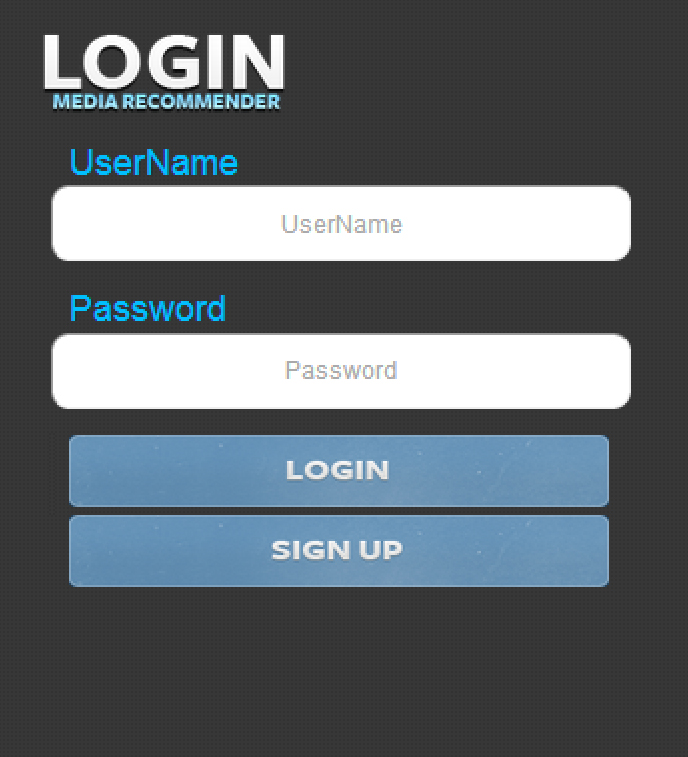
\includegraphics[width=.9\linewidth]{Images/new-login.jpg}
  \caption{Login}
  \label{fig:new-login}
\end{subfigure}%
\begin{subfigure}{.5\textwidth}
  \centering
  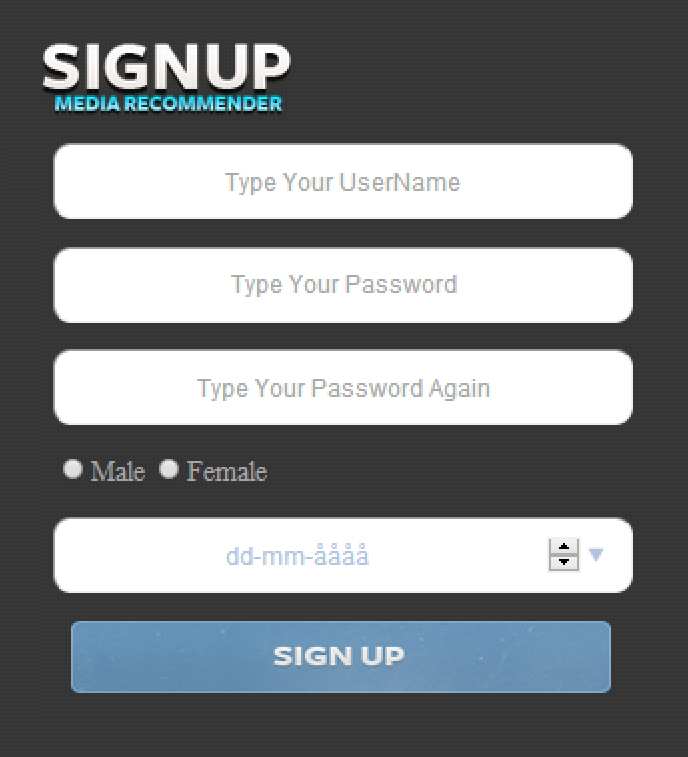
\includegraphics[width=.9\linewidth]{Images/new-signup.jpg}
  \caption{Signup}
  \label{fig:new-signup}
\end{subfigure}
\caption{Redesign of Login and Signup}
\label{fig:login-signup}
\end{figure}



After creating an user and being logged in to the website you’ll be directed to the frontpage. Compared to the old design of the website figure \ref{CurrSite}, on page \pageref{CurrSite}, there have been added a search bar and an ability to specify which media and a rating ability. In the searh bar you can search for a specific media and if you click enter right after you write something in the search bar it will directly do the a search. The rating is made out radio buttons up to 10 which makes it easier for the design when the media is right under like a list where you have the ability to have the rating right over it. The choice for 10 for rating is because it converts this to 5-star rating in medialist. Every rating is a half star, example rating on 1 will be a half star and rating on 5 will be 2 and a half star. So mathematically rating divided by 2 will be the out put of the stars.

On the right side of figure \ref{fig:new-frontpage} you will be able to see that movies, games and books have been combined into one button called recommendation compared to the old design figure \ref{CurrSite} on page \pageref{CurrSite}. The recommendation button is chosen to be red according to figure \ref{Colors} it gives a hot feeling like what’s hot, and according to empower-yourself-with-color-psychology.com it means that you are ready to take action. 
If you rate and add a media it will give you a notification saying: “Added to your medialist”, so the user will know where his/her media will be added to. But this way isn't the most optimal way, since you won't know this from the beginning that you can click on the media and it will add to your medialist.

\begin{figure}[H]
\centering
\begin{subfigure}{.5\textwidth}
  \centering
  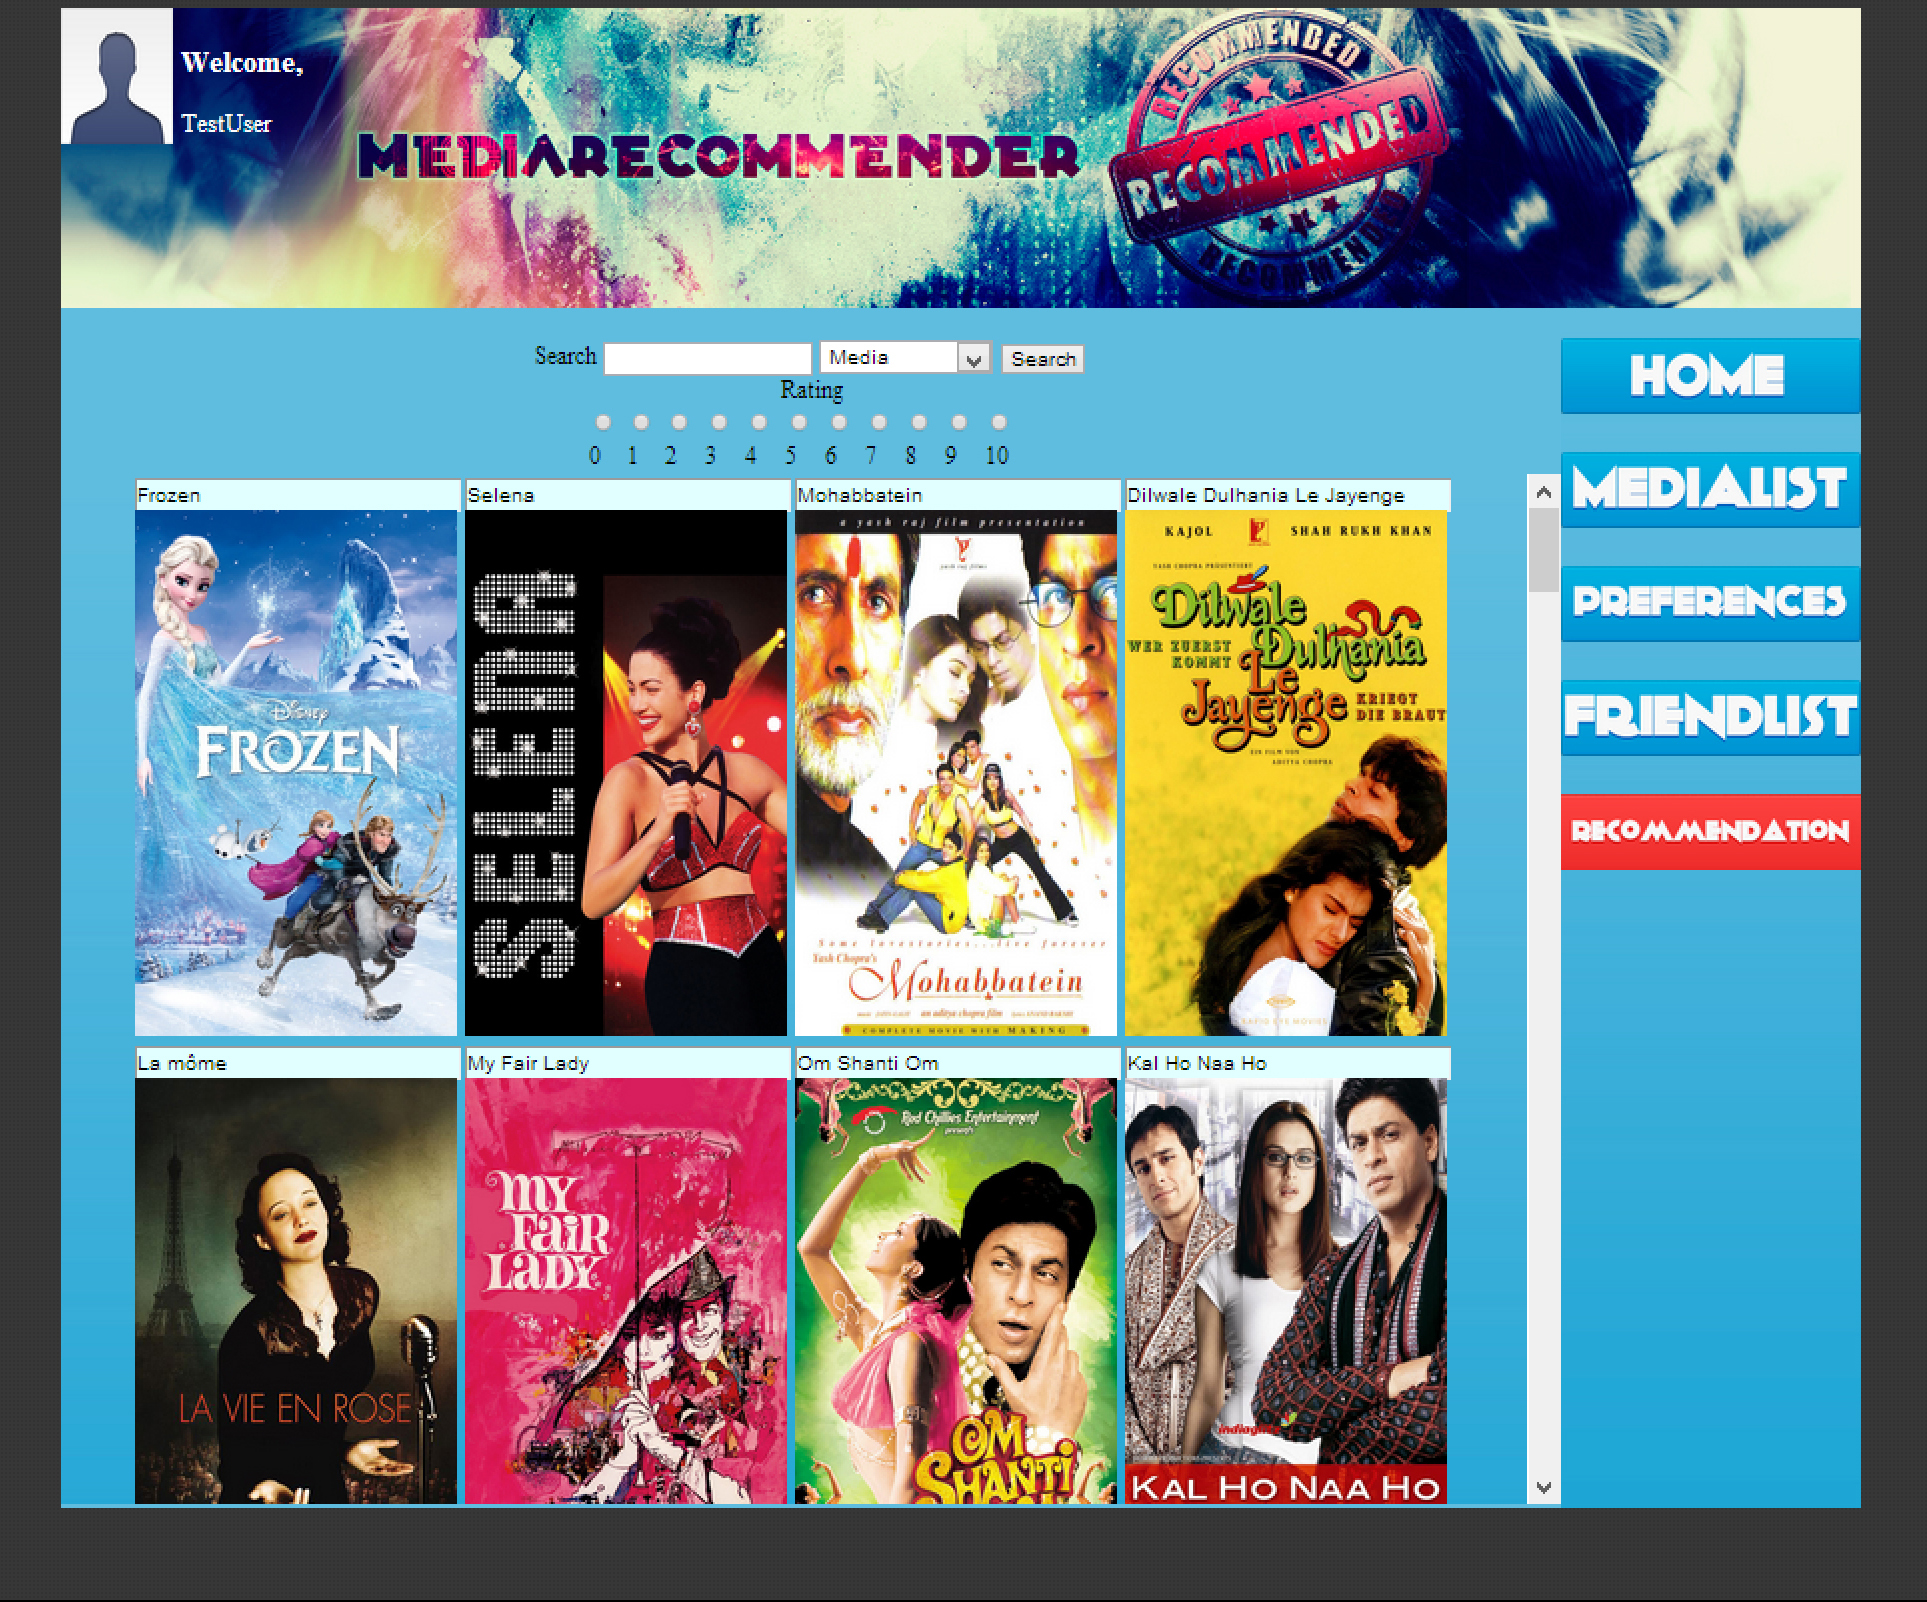
\includegraphics[width=.9\linewidth]{Images/new-home.jpg}
  \caption{Frontpage}
  \label{fig:new-frontpage}
\end{subfigure}%
\begin{subfigure}{.5\textwidth}
  \centering
  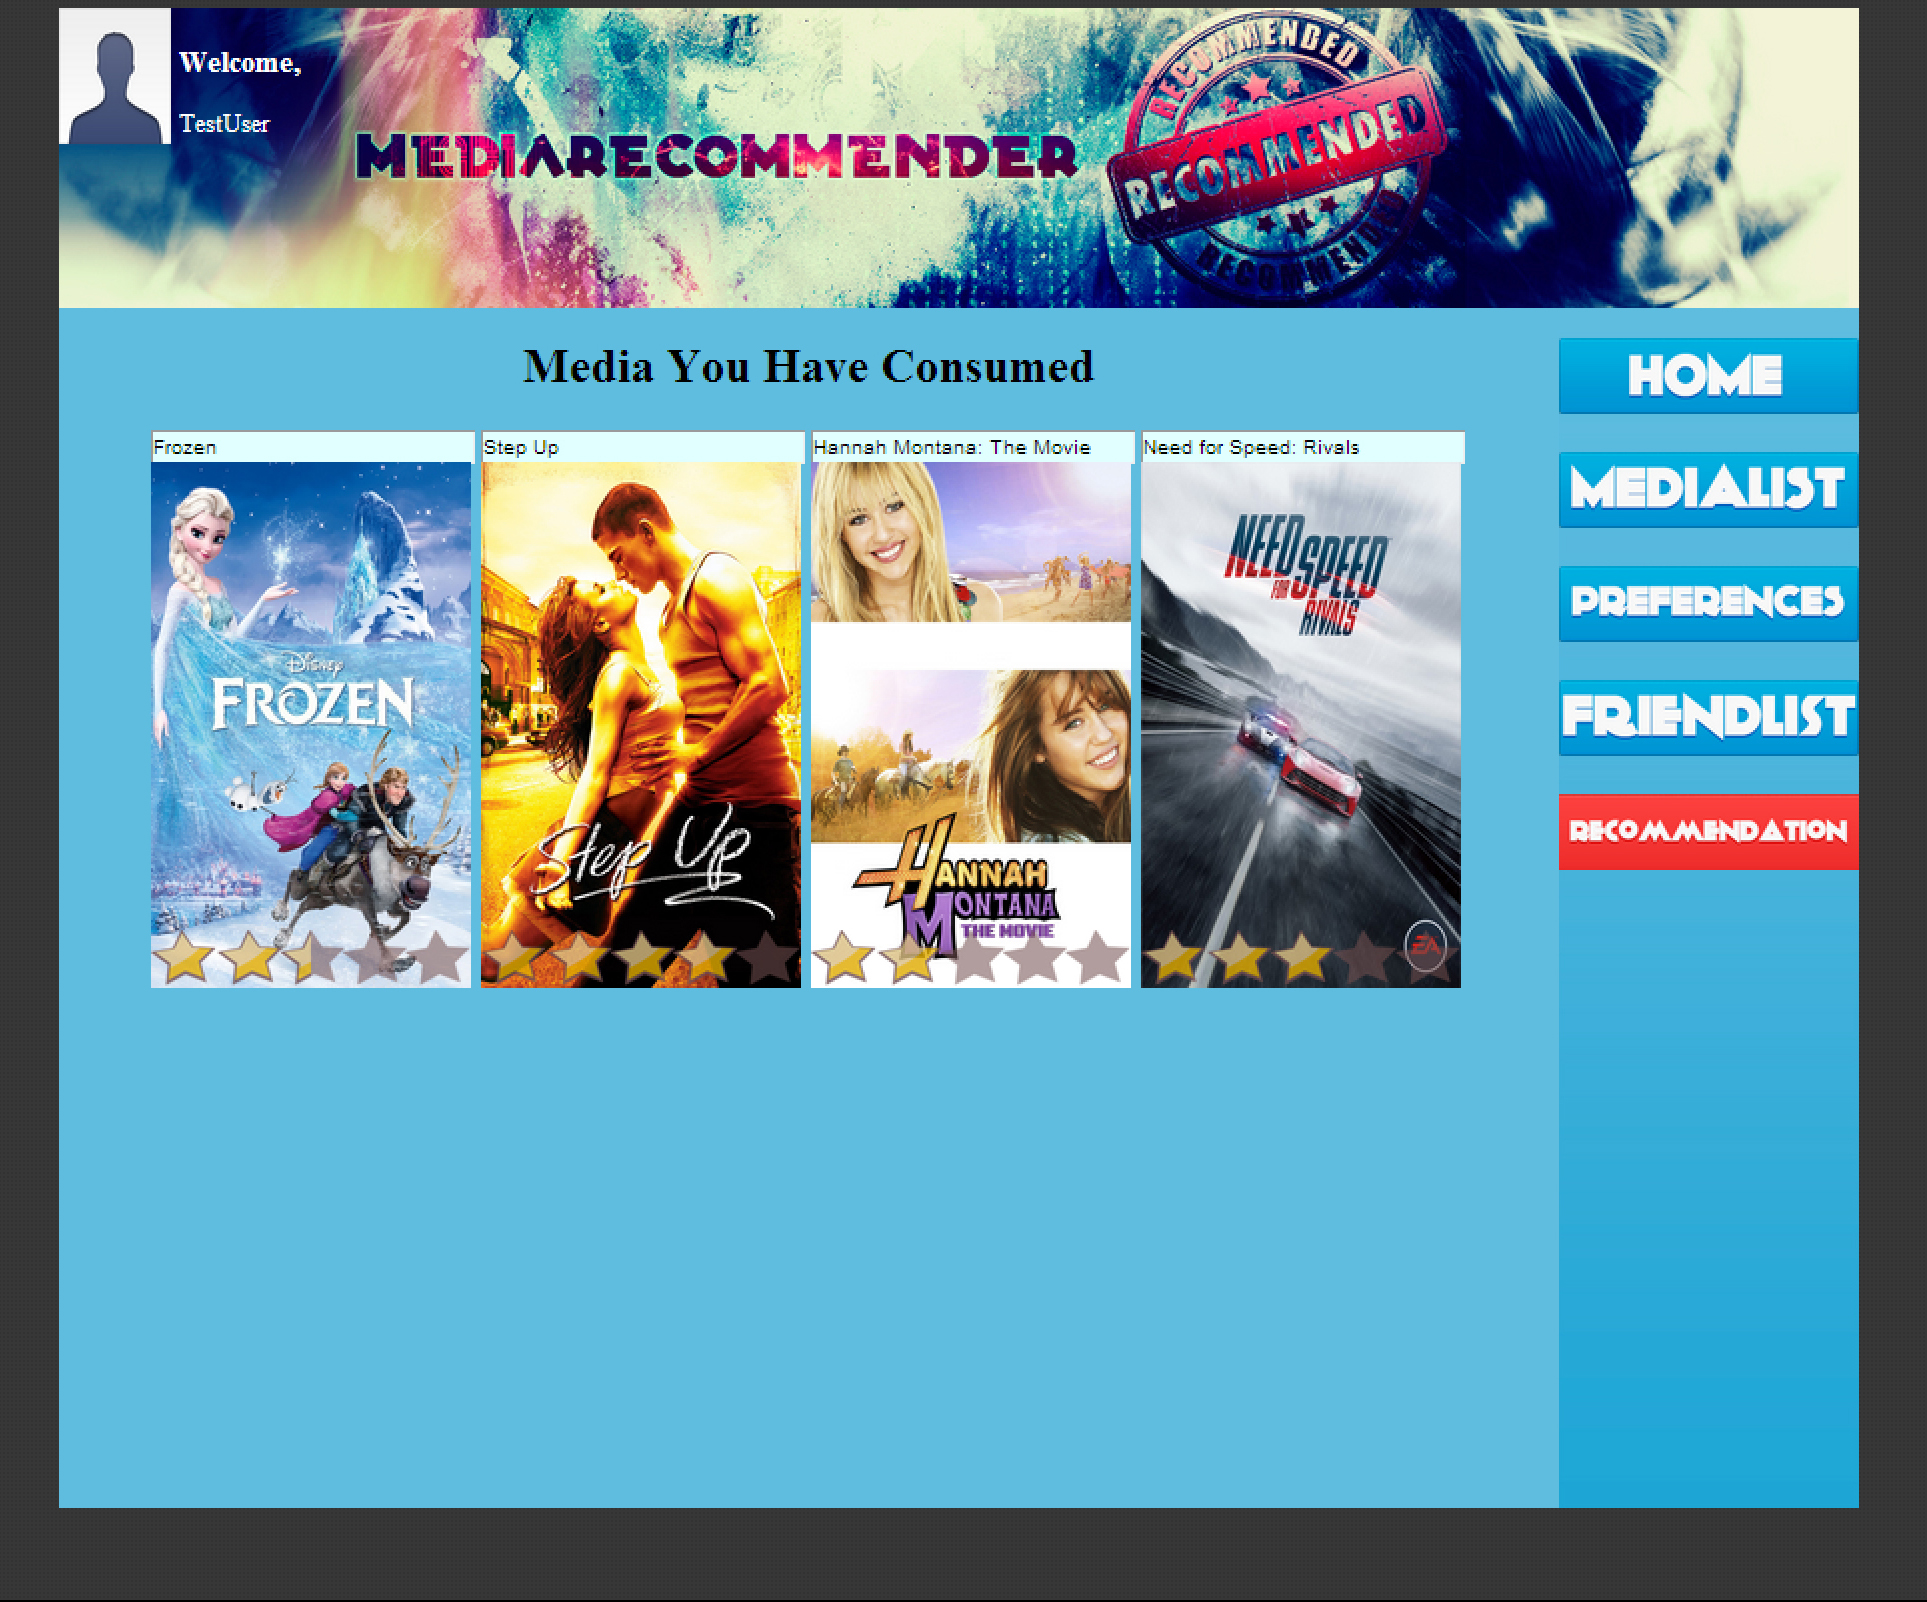
\includegraphics[width=.9\linewidth]{Images/new-medialist.jpg}
  \caption{Medialist}
  \label{fig:new-medialist}
\end{subfigure}
\caption{Redesign of frontpage and medialist}
\label{fig:front-media}
\end{figure}

On the medialist, figure \ref{fig:new-medialist} page you will see all the medias you have added to the medialist and your rating will be shown on the media cover. If you click on the media there will be shown a confirmation notification saying: “Are you sure you want to remove this media?”. Whether the user accept or not the media will be removed from the users medialist. Again this is not the optimal way to do, because the user won't be able to know this from the beginning and there isn't any information about this.

On the preference page is where all the genres. The user can specify what’s he/she is into. This will affect the output of the recommendation.

On the recommendation page is where the user gets his/her recommendation done by the collaborative and content based algorithms. The output of the recommendation is compared with your medialist and all other users medialist.

The design have some kind colors, which again are black, white, blue and red, to make the user feel more comfortable. The design of the website is simple. There isn't any information on the website about clicking on the media and it will do commands like adding or removing.
